\documentclass[10pt,a4paper]{article}
\usepackage[utf8]{inputenc}
\usepackage[T1]{fontenc}
\usepackage{graphicx}
\usepackage{amsmath}
\usepackage{float}
\graphicspath{{./figures/}}

\title{MA332 Project 1}
\author{Ben Raivel}
\begin{document}
	\maketitle
	\section{Introduction}
	Newton's Method is a numerical root-finding algorithm. To find a root $ f(x_\star) = 0 $, the algorithm uses $f$, its derivative $f^\prime$, and some initial value $x_0$. Starting at $x_0$ the algorithm iterates, with the  $ n+1^\text{th} $ approximation given by:
	$$ x_{n+1} = x_n - \frac{f(x_n)}{f^\prime(x_n)} $$

	In most cases, the approximation generated by Newton's Method will be quite accurate within a few iterations.
	\section{Failure to Converge}
	Depending on the function and starting value, Newton's Method may not converge. There are several circumstances under which this happens.
	
		\subsection{Converges to a Cycle}
		
		In the case of certain functions which have a local minimum or maximum but no root on an interval, Newton's Method can get stuck in a cycle around the minimum/maximum.
		
		Consider the function $ g(x) = x^3 - 2x  + 2 $, which has one root: $ g(-1.769) \approx 0$. Newton's method with $g(x)$ gives the $ n+1^\text{th} $ approximation:
		$$ x_{n+1} = x_n - \frac{x_n^3 - 2x_n + 2}{3x_n^2 - 2} $$
		Observe that if $x_n = 0$:
		$$ x_{n+1} = 0 - \frac{2}{-2} = 1 $$
		And if $x_n = 1$:
		$$ x_{n+1} = 1 - \frac{1 - 2 + 2}{3 - 2} =  0 $$		
		If given either 0 or 1 as a starting value, Newton's Method will cycle infinitely.  These are not the only starting points for which Newton's Method fails to converge. Figure 1 shows the sub-intervals on [-3, 3] where Newton's Method does not find a root.
		
		\begin{figure}[H]
			\centering
			\caption{Starting values that do not converge for $ g(x)  = x^3 - 2x + 2 $}
			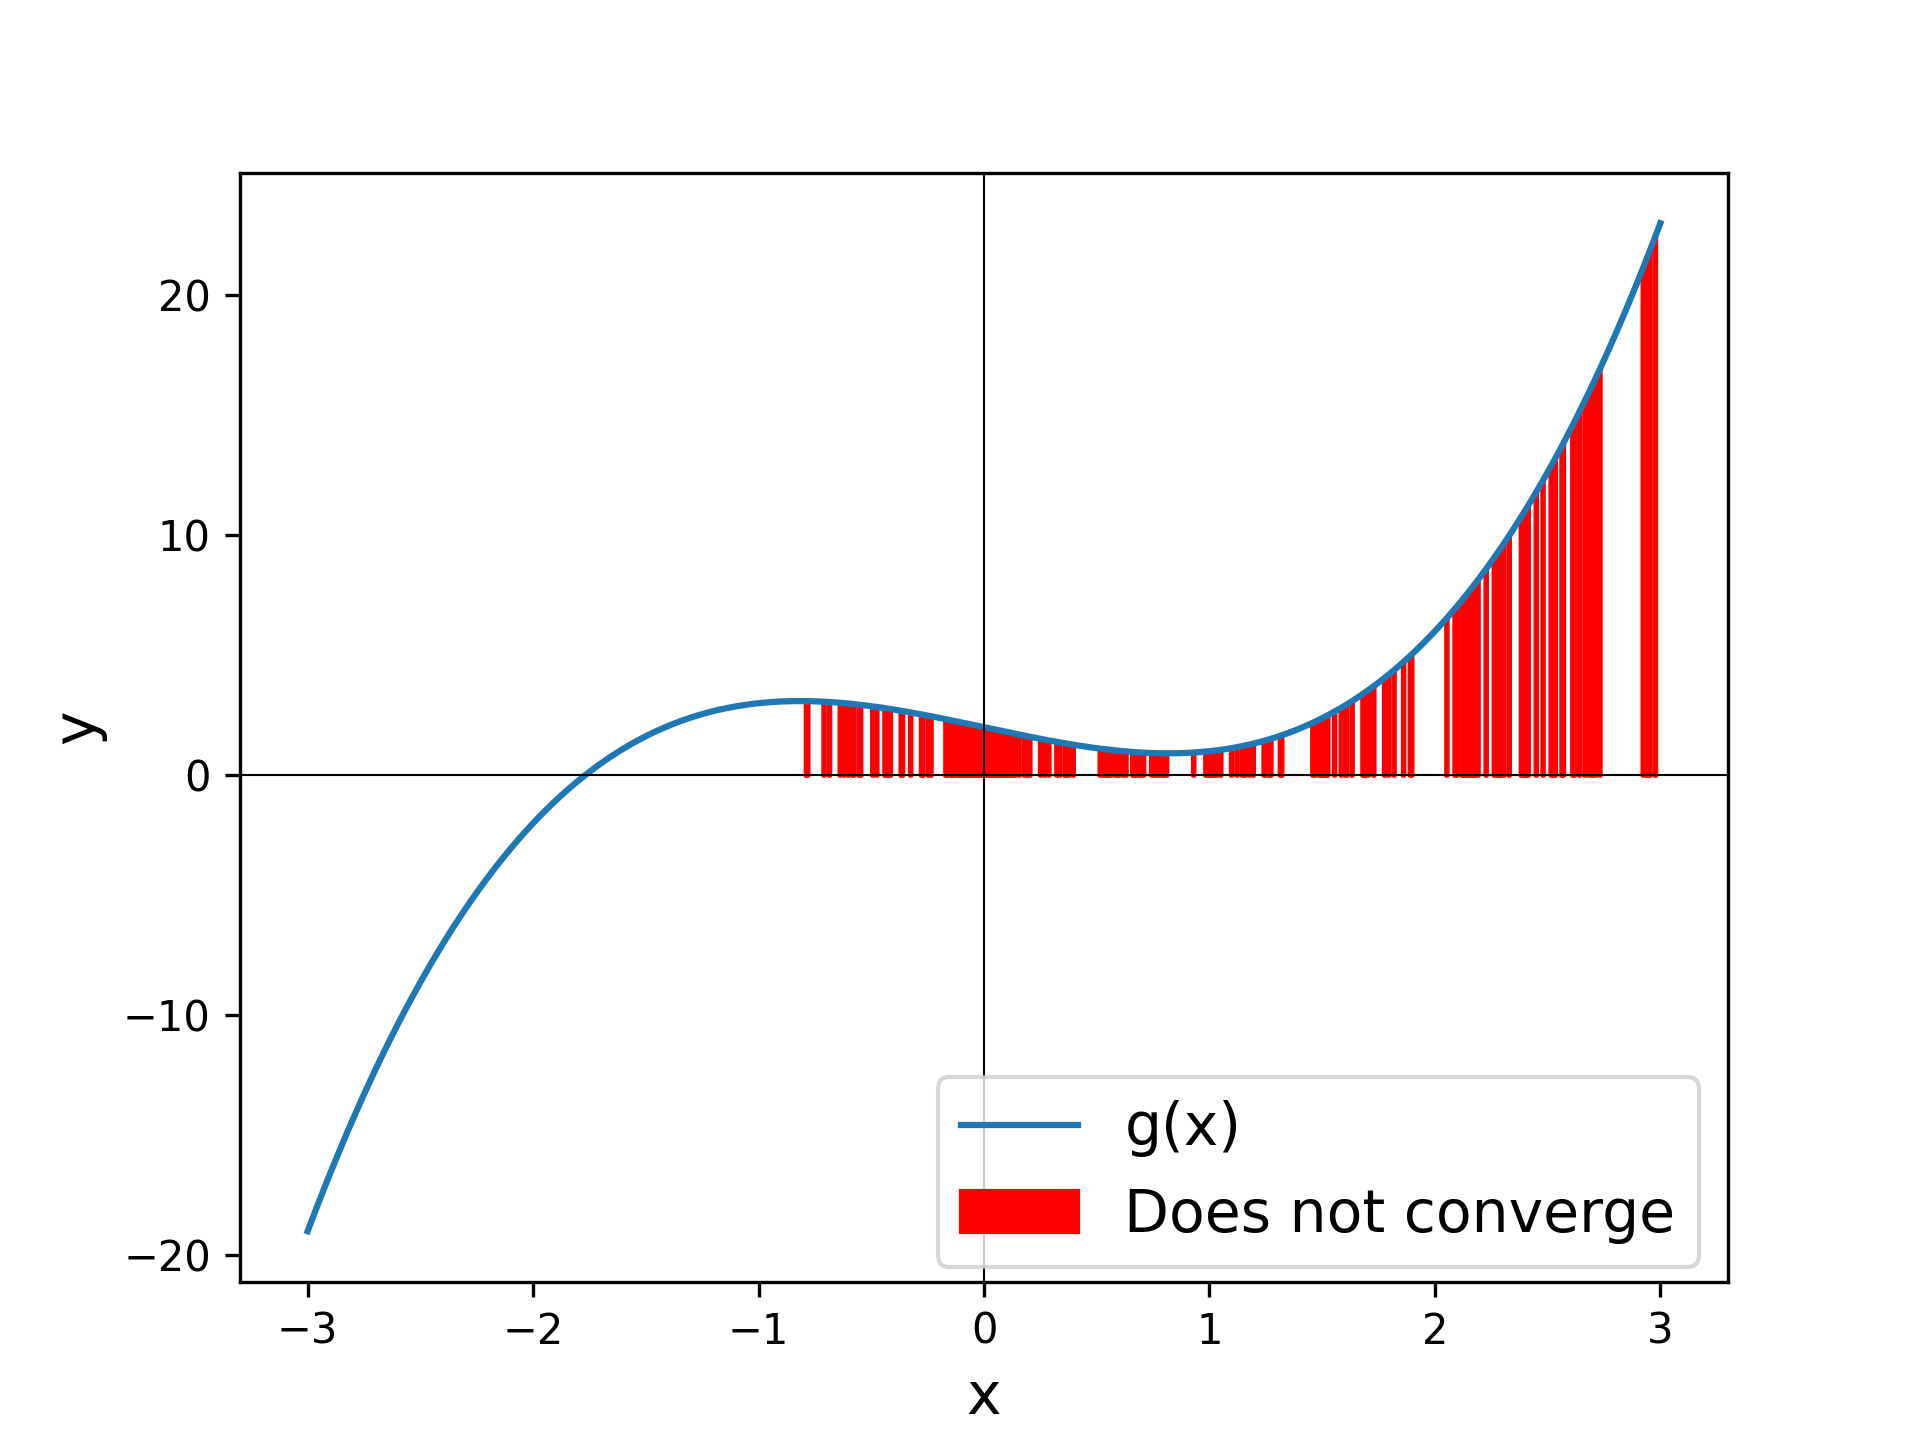
\includegraphics[scale=0.5]{figure1}
		\end{figure}
	
		To see what happens for non-convergent starting values besides 0 and 1, look at the series of approximations generated by one of these starting points ($x=0.1$):
		\begin{table}[H]
			\centering
			\caption{Newton's Method on $g(x)$ after $n$ iterations starting at 0.1}
			\begin{tabular}{ c | l }
				\hline
			 	$n$ & $x_n$ \\
			 	\hline\hline
			 	0 & 0.1\\
			 	1 & 1.014213\\
			 	2 & 0.079656\\
			 	3 & 1.009099\\
			 	4 & 0.052227\\
			 	5 & 1.003965\\
			 	6 & 0.023329\\
			 	7 & 1.000804\\
			 	8 & 0.004807\\
			 	9 & 1.000035\\
			\end{tabular}
		\end{table}
		 Table 1 shows that the series of approximate roots for non-convergent starting points besides 0 and 1 asymptotically approaches the 0-1 cycle.

		\subsection{Diverges}
		Newton's Method will also encounter issues if the derivative does not exist at the root. Consider the function $h(x) = x^{1/5}$. Newton's Method gives the $ n+1^\text{th} $ approximation of the root:
		$$ x_{n+1} = x_n - 5\frac{x_n^{1/5}}{x_n^{-4/5}} = x_n - 5x_n = -4x_n$$
		Each $x_{n+1}$ will have the opposite sign to $x_n$ and be four times further from the root. The output of the Newton's Method implementation used for this project confirms this:
		\begin{table}[H]
			\centering
			\caption{Newton's Method on $h(x) = x^{1/5}$ after $n$ iterations starting at 1}
			\begin{tabular}{c | r}
				\hline
				$n$ & $x_n$\\
				\hline\hline
				0 & 1\\
				1 & -4\\
				2 & 16\\
				3 & -64\\
				4 & 256\\
				5 & -1024\\
				6 & 4096\\
			\end{tabular}
		\end{table}
	\section{Basins of Attraction}
	For a given root $ f(x_\star) = 0$, the \emph{basin of attraction} is the set of starting values $ x_0 $ for which Newton's Method on $f$ will converge to $ x_\star $.
	
		\subsection{Real-Valued Functions}
		Consider the function $ g(x) = (x - 1)(x + 3) $
		\begin{figure}[H]
			\centering
			\caption{Basins of convergence for $g(x) = (x - 1)(x + 3)$}
			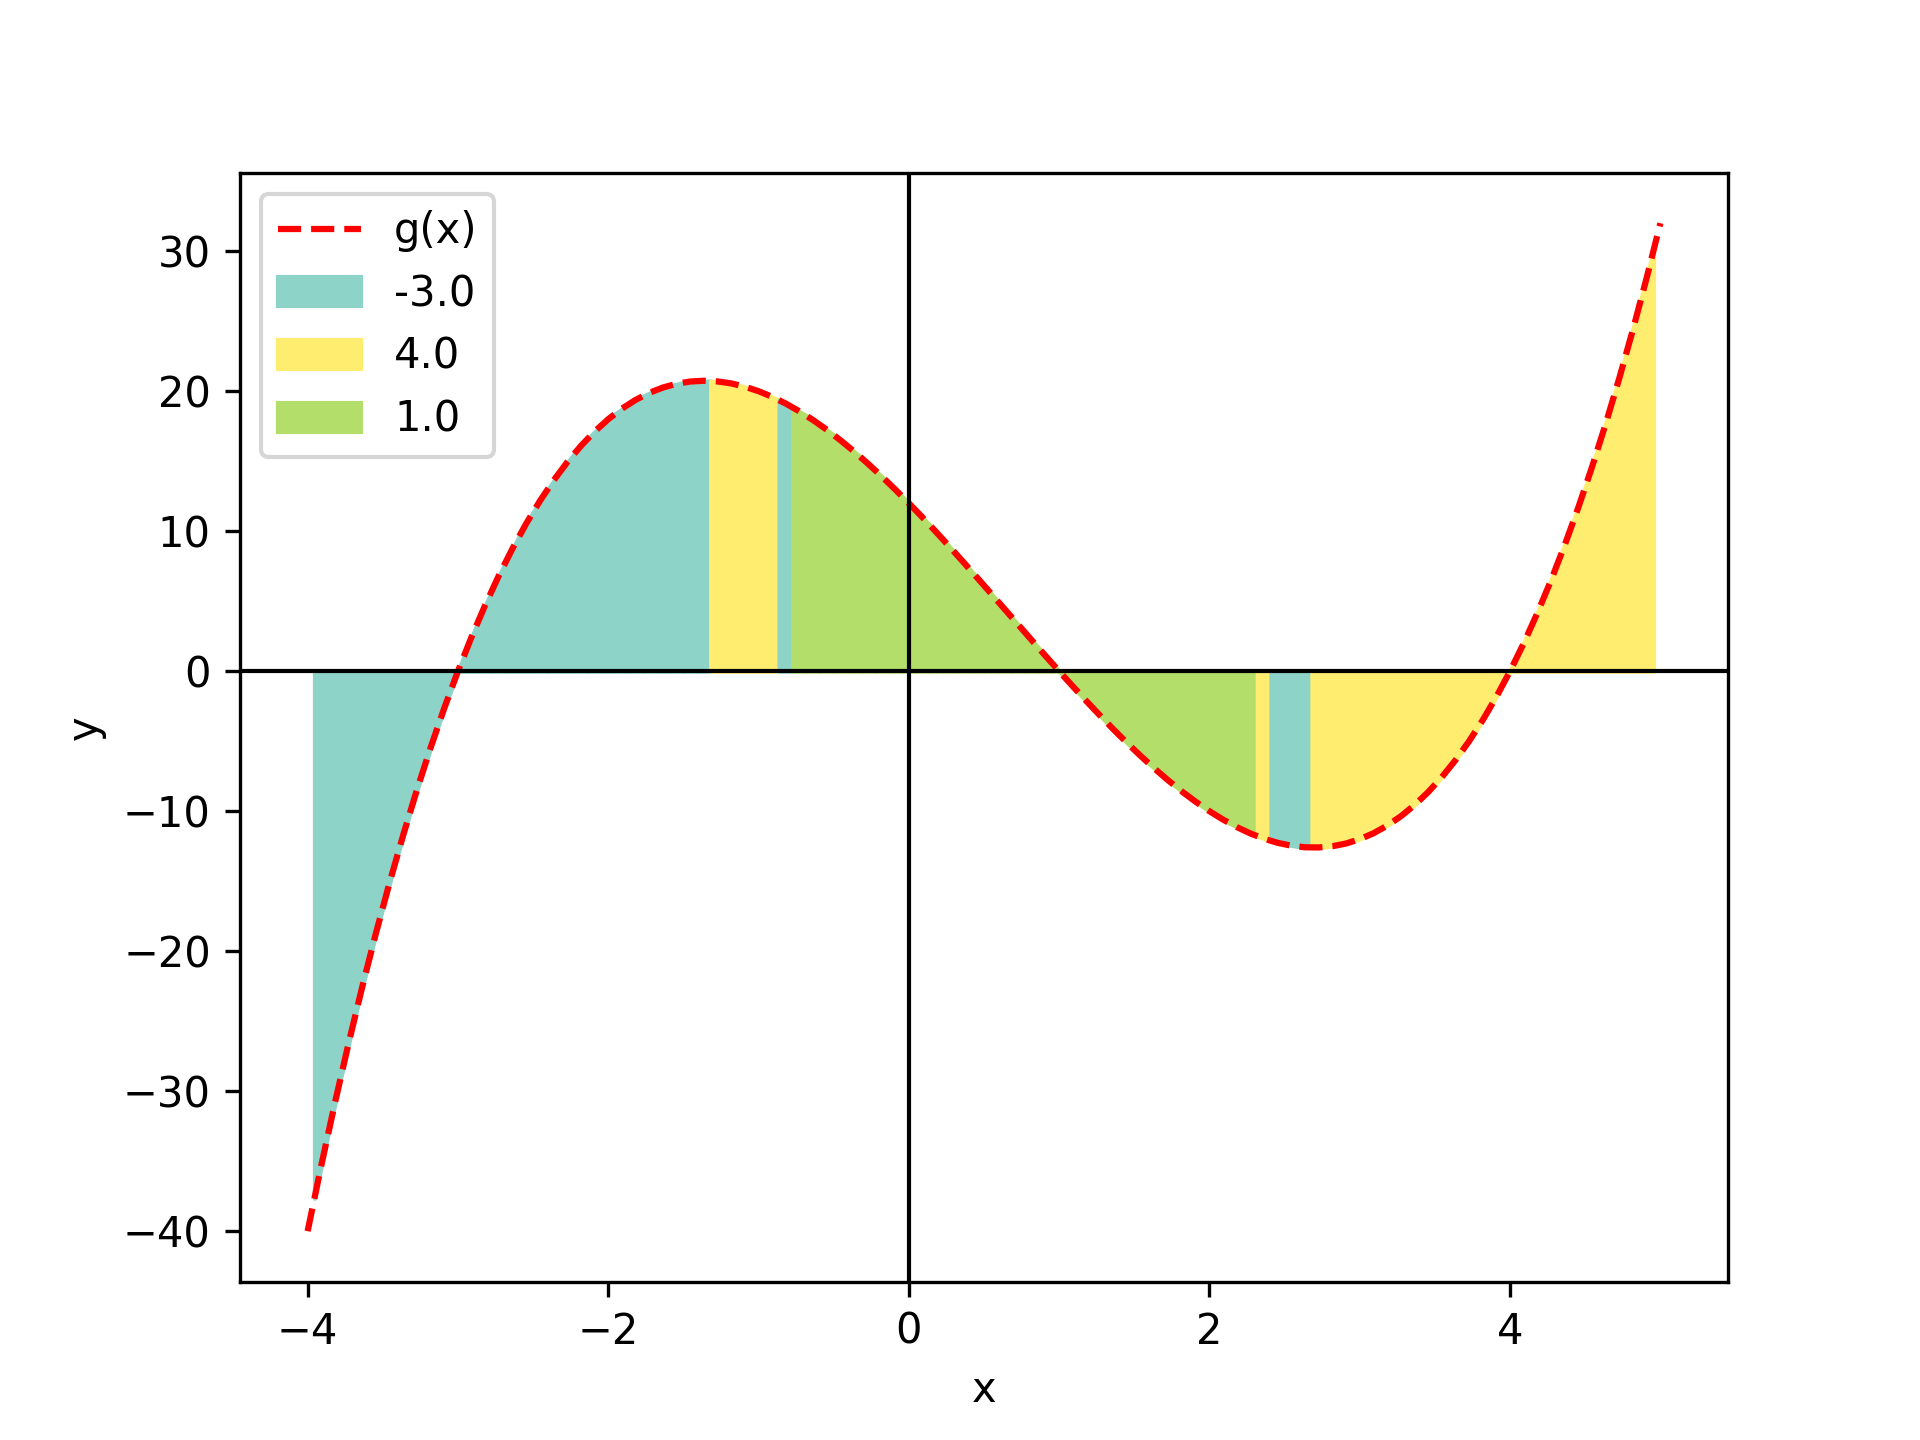
\includegraphics[scale=0.5]{figure2}
		\end{figure}
		For a second-degree polynomial with two roots the basins are very simple, meeting at the minimum/maximum of the function and extending out to infinity. Introducing a third root has an interesting effect. Consider the function $ h(x) =  (x - 4)(x - 1)(x + 3)$. Figure 3 shows the basins of convergence for the three roots:
		\begin{figure}[H]
			\centering
			\caption{Basins of convergence for $h(x) = (x - 4)(x - 1)(x + 3)$}
			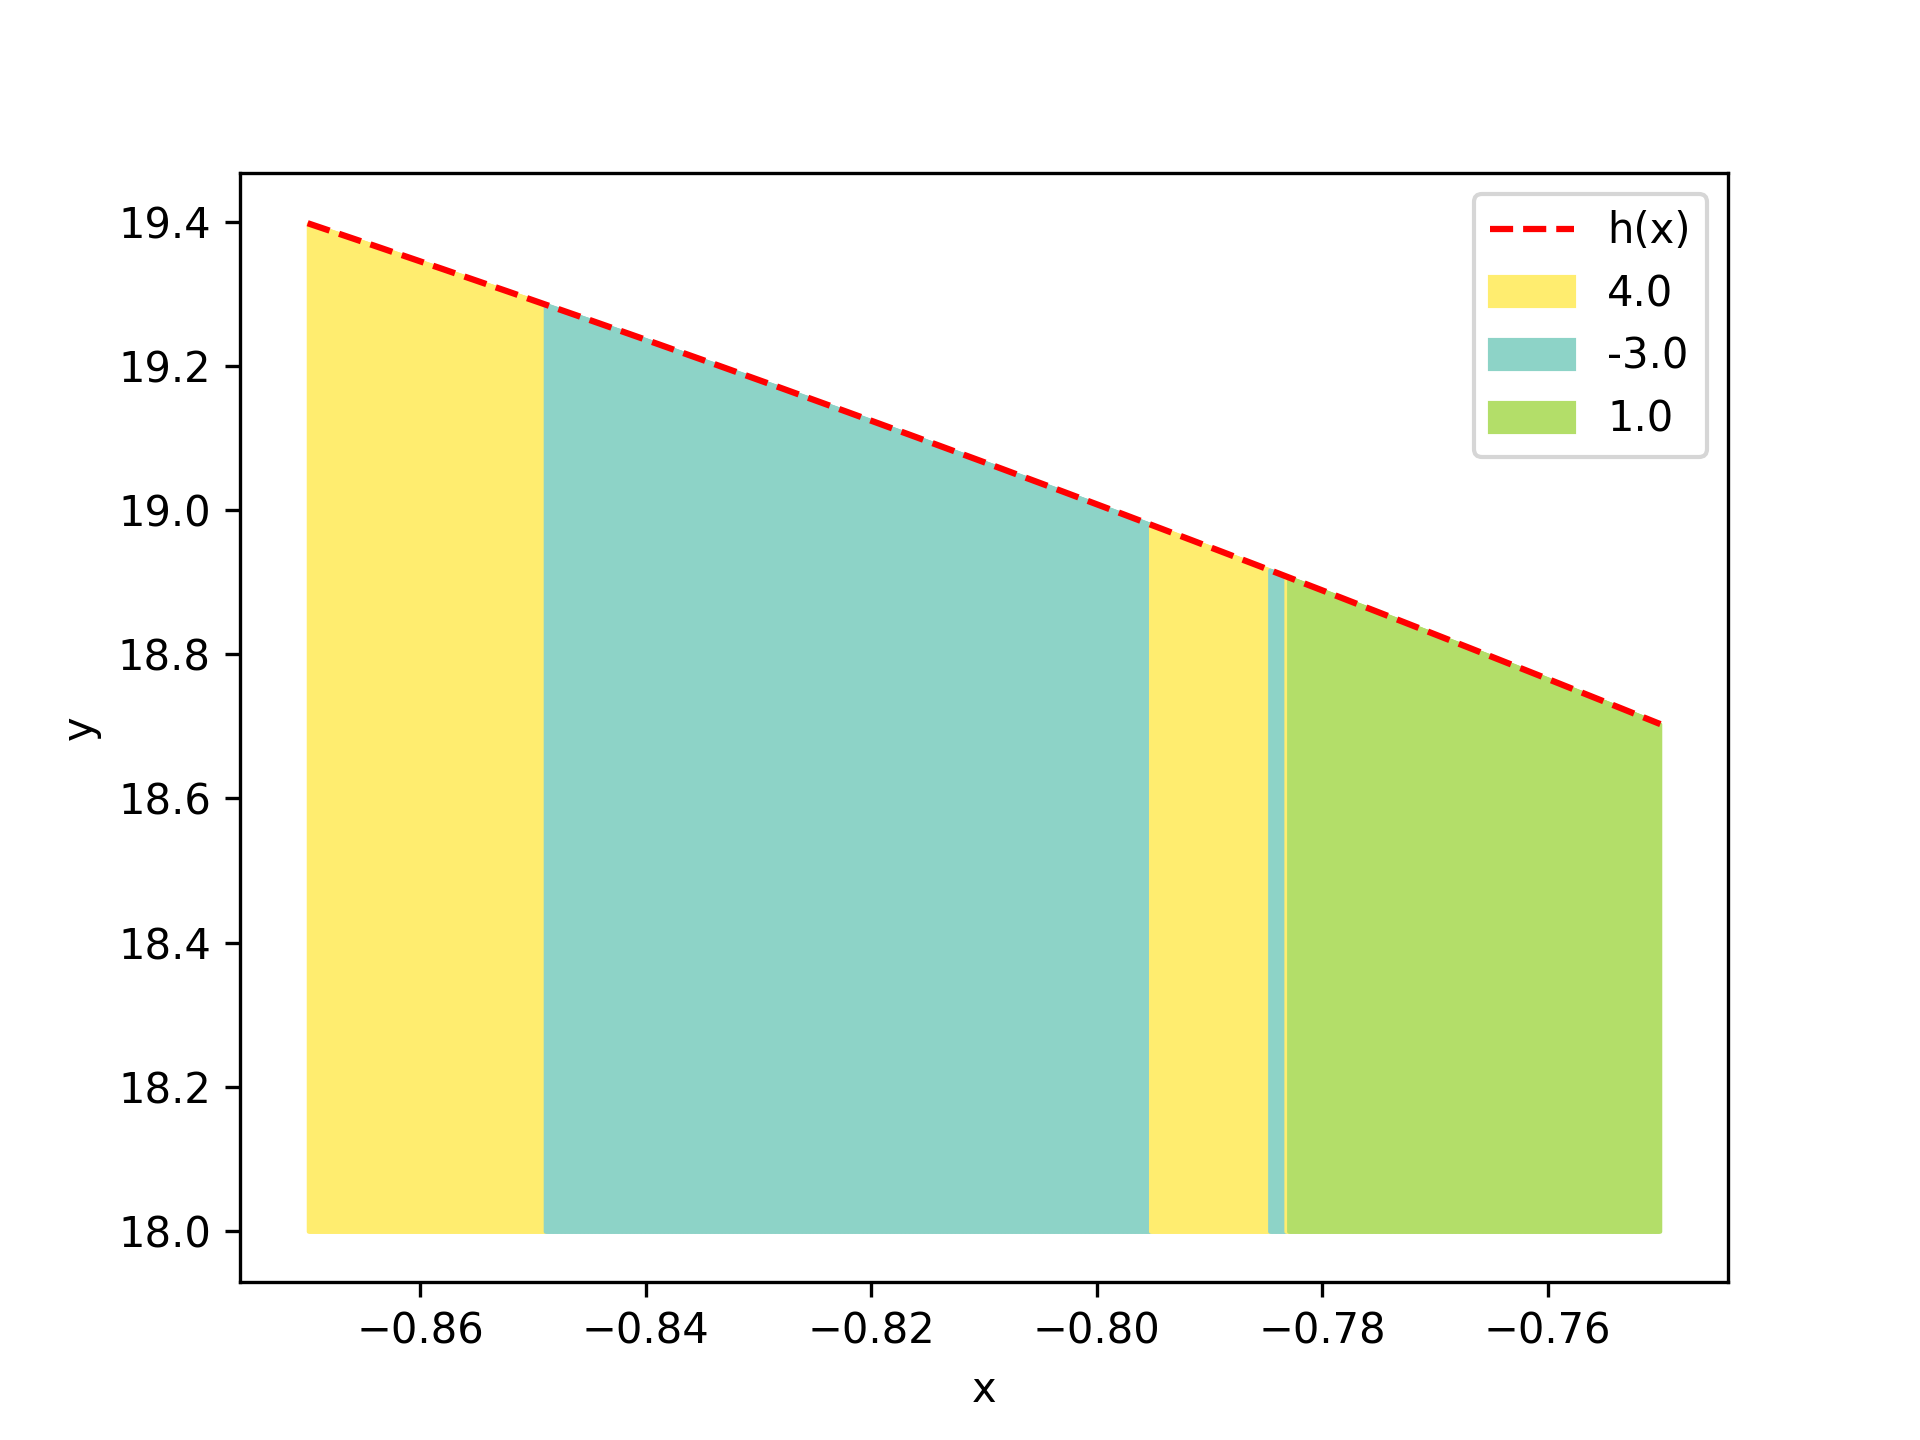
\includegraphics[scale=0.5]{figure3}
		\end{figure}
		Two of the three basins are no longer contiguous. When the derivative is small compared to the value of the function (around $x=-1.5$ and $x=2.5$ in Figure 2), the approximation will change by a large amount. This means Newton's Method can jump over the middle basin and find a root far from where it started. A subset of those jumps will land in regions which jump back again (and a further subset will jump a third time, etc.)
		\begin{figure}[H]
			\centering
			\caption{Zooming in shows the fractal pattern of the basins}
			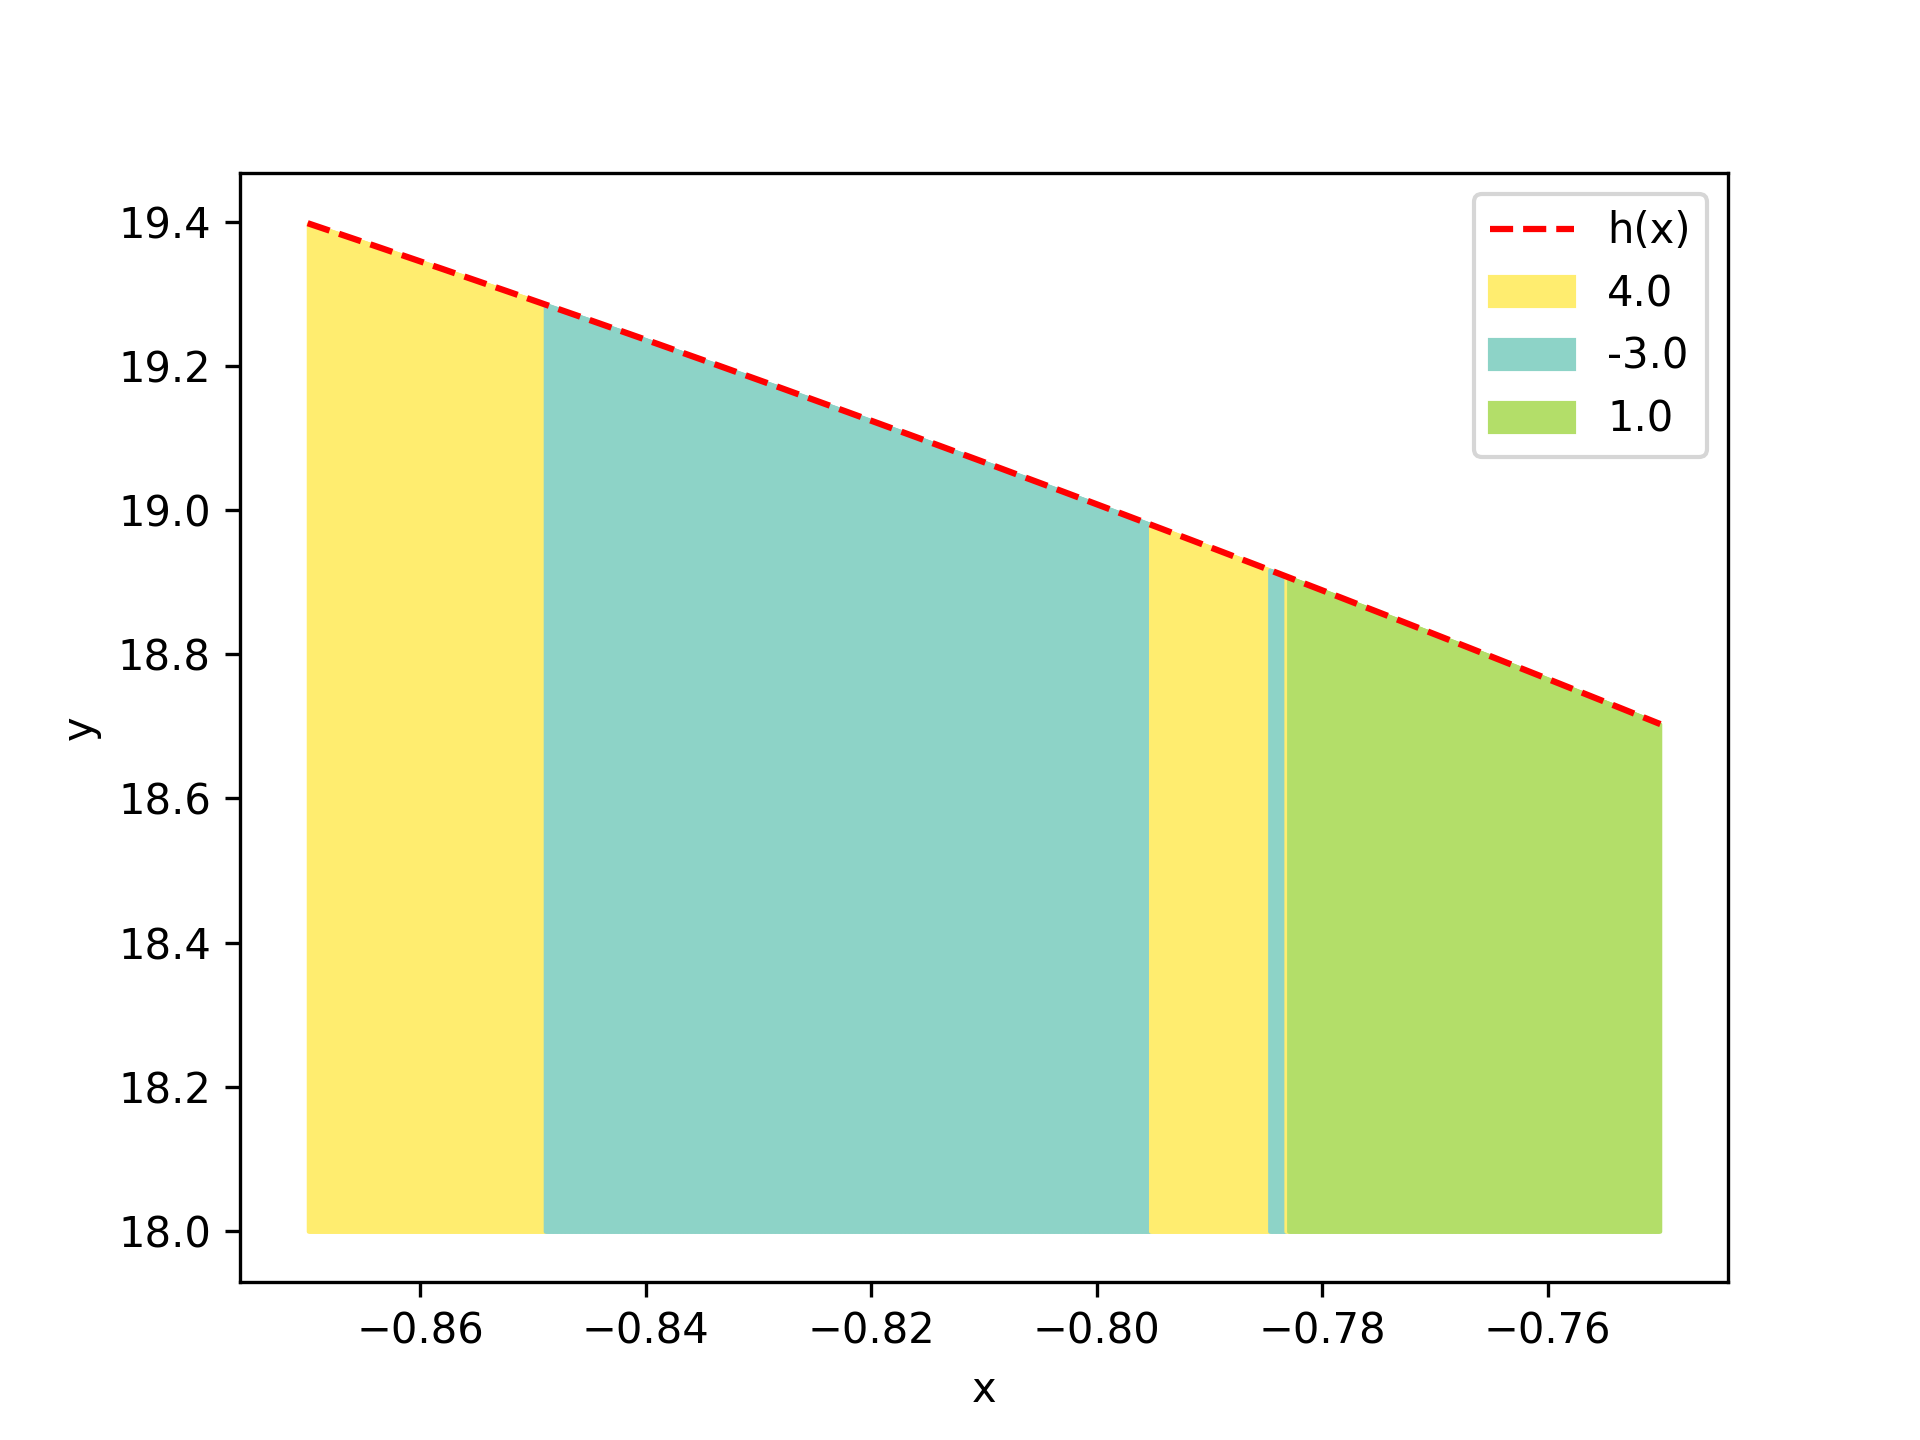
\includegraphics[scale=0.5]{figure4}
		\end{figure}
	
		\subsection{Complex-Valued Functions}
		Extending this to complex-valued functions adds another "dimension" along which basins can interface with each other. The one-dimensional fractal behavior visible in Figure 4 becomes much more intricate when visualized on the complex plane. 
		\begin{figure}[H]
			\centering
			\caption{Basins of convergence for $f(z) = z^3 - 1$ on the complex plane $a+bi$}
			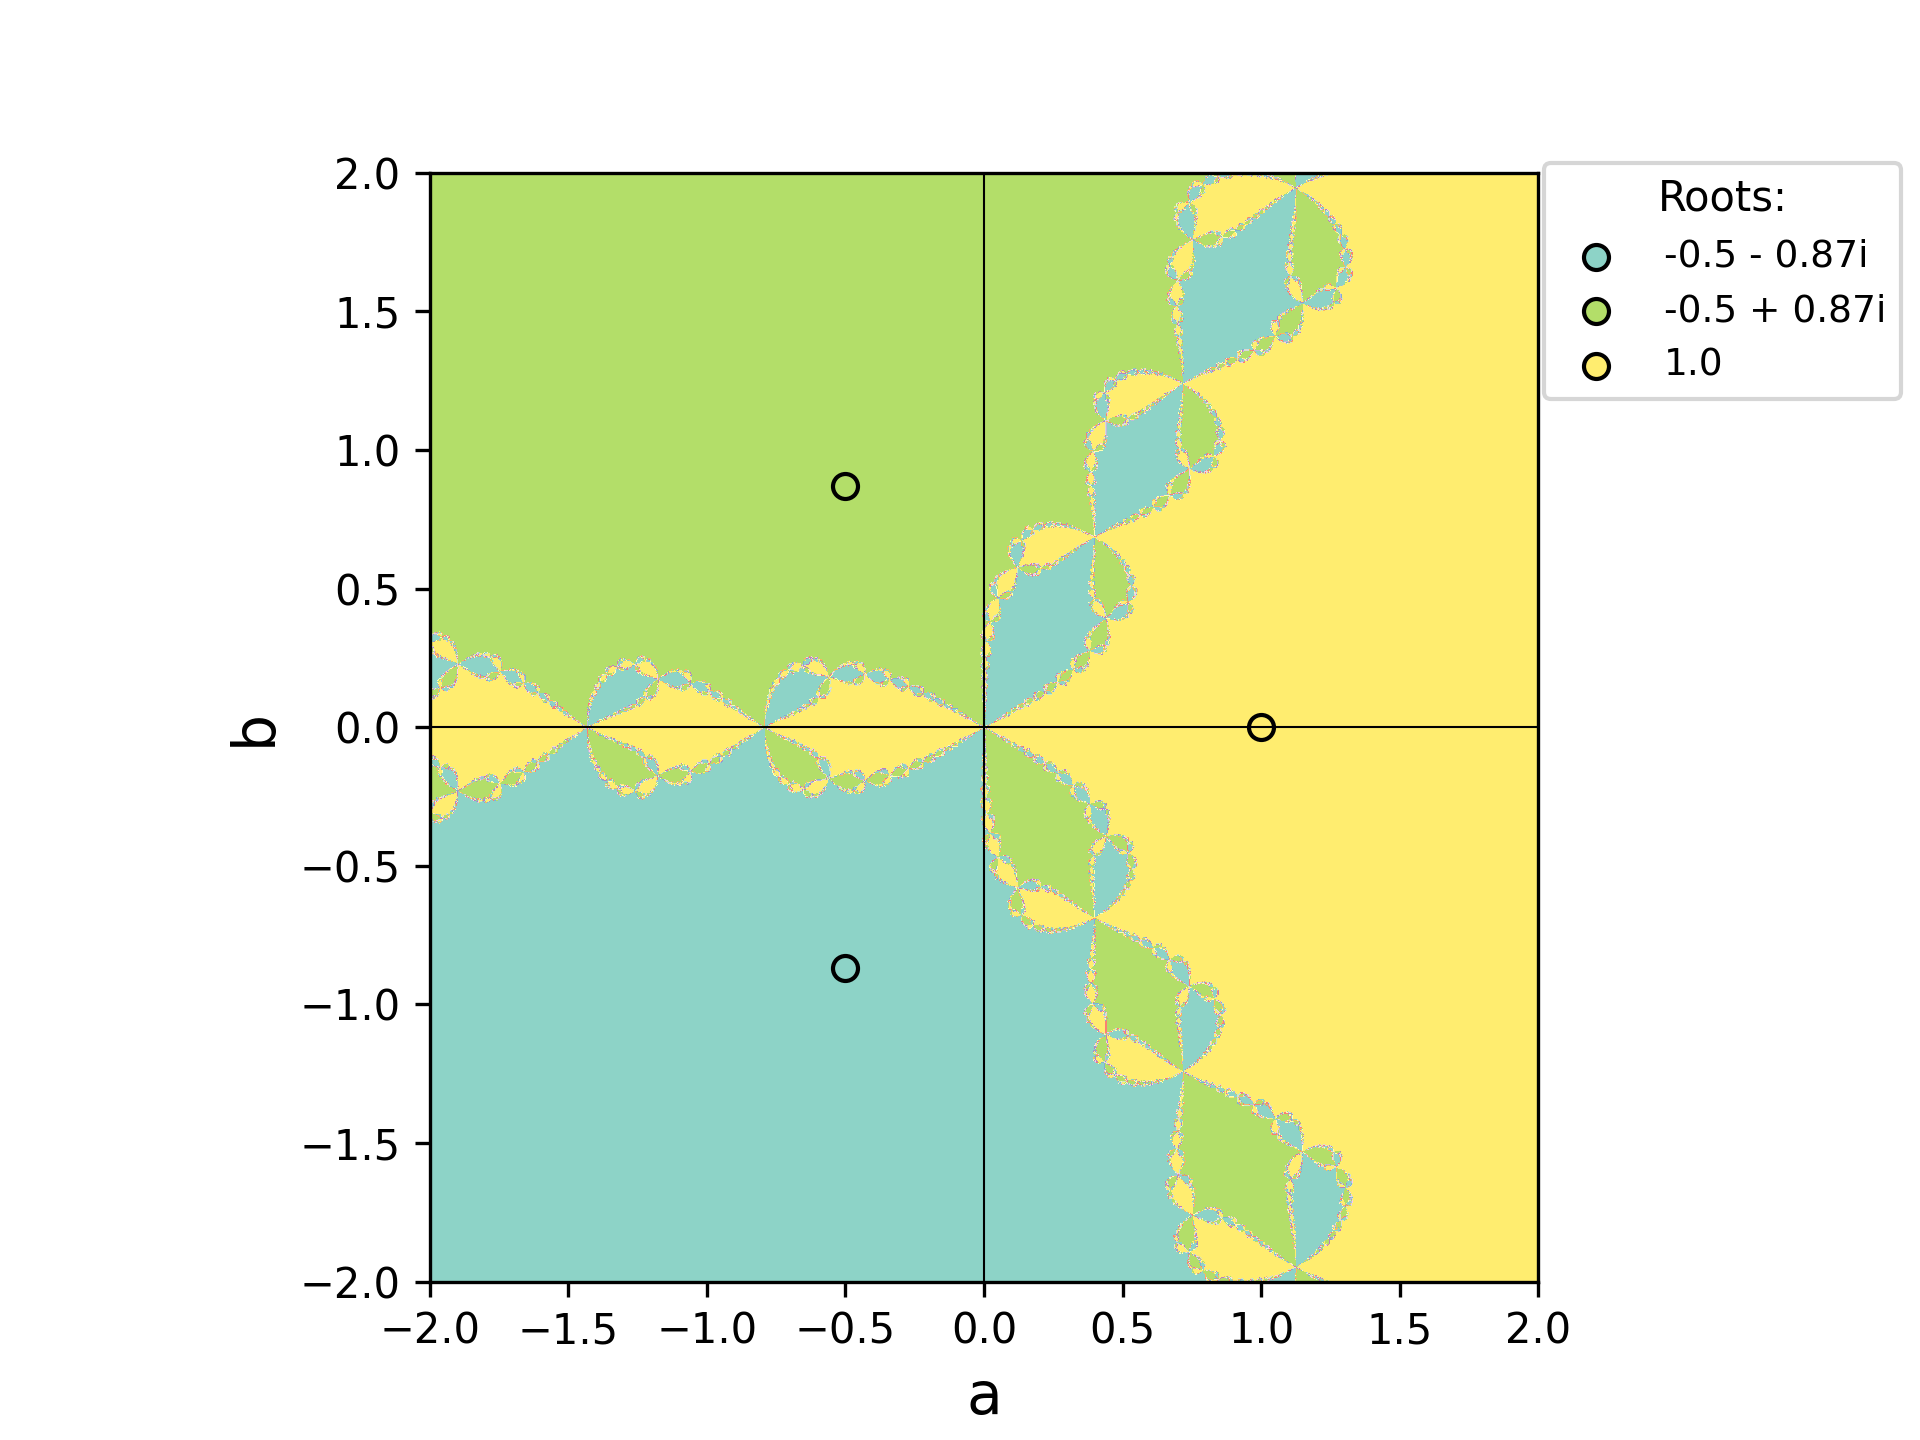
\includegraphics[scale=0.5]{figure5}
		\end{figure}
		$f(z)=z^3-1$ is not unique, $g(z)=z^5 - z^3 -2$ produces a similar (though less symmetrical) image:
		\begin{figure}[H]
			\centering
			\caption{Basins of convergence for $g(z) =z^5 - z^3 -2$ on the complex plane $a+bi$}
			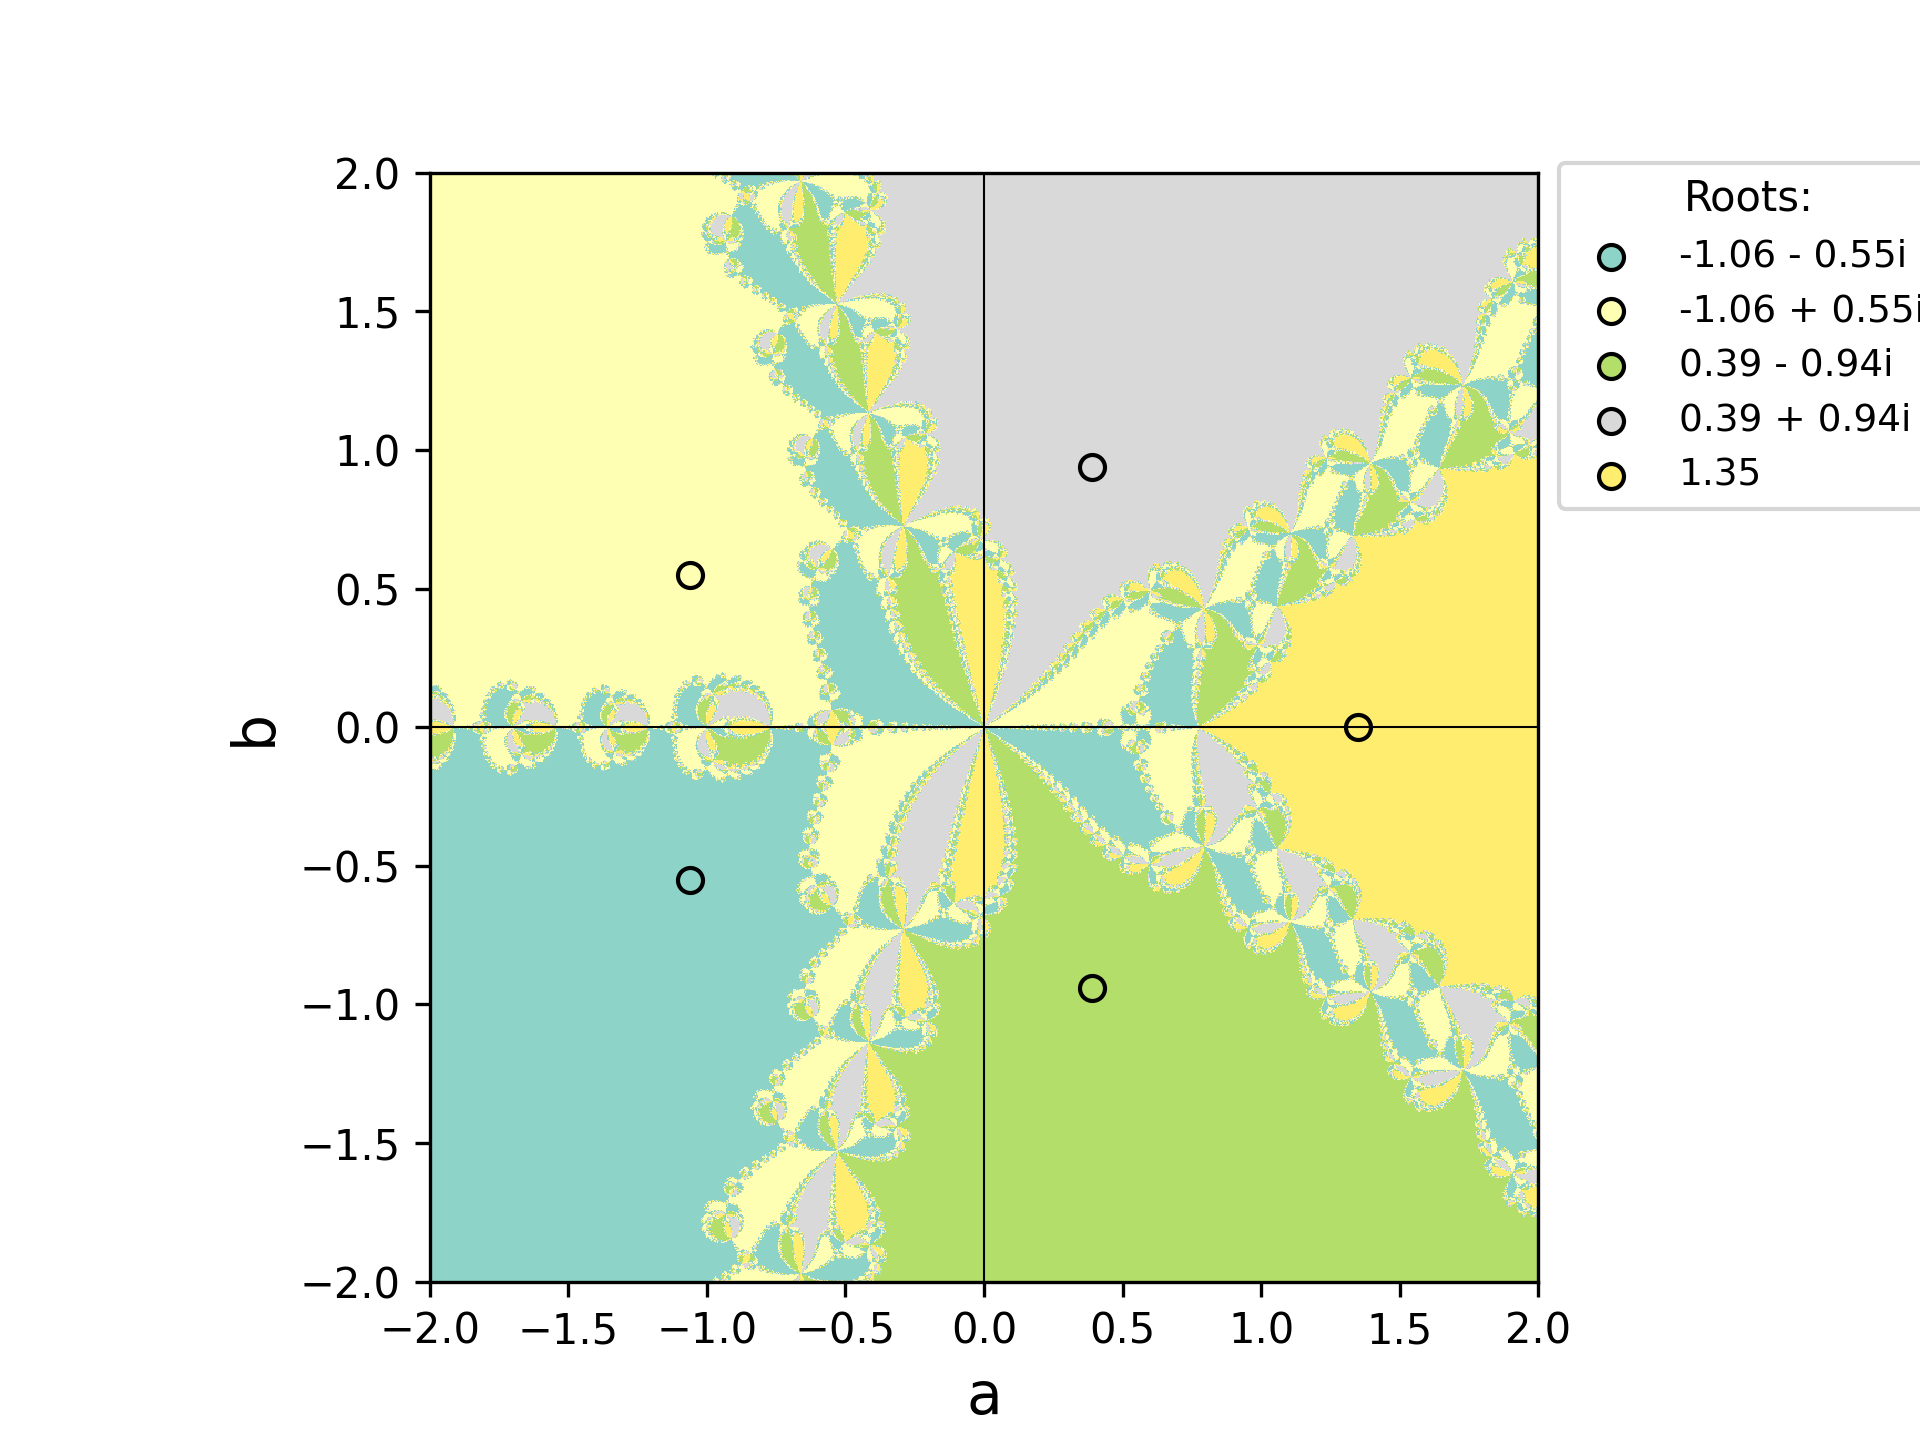
\includegraphics[scale=0.5]{figure6}
		\end{figure}
		The roots do not need to be complex, as long as there are at least three the basins will form a fractal. Consider again the function $h(x) =  (x - 4)(x - 1)(x + 3)$, with real basins of convergence shown in Figure 3. The basins are shown again in Figure 7, this time in the complex plane.
		
		\begin{figure}[H]
			\centering
			\caption{Basins of convergence for $h(x) =  (x - 4)(x - 1)(x + 3)$ on the complex plane $a+bi$}
			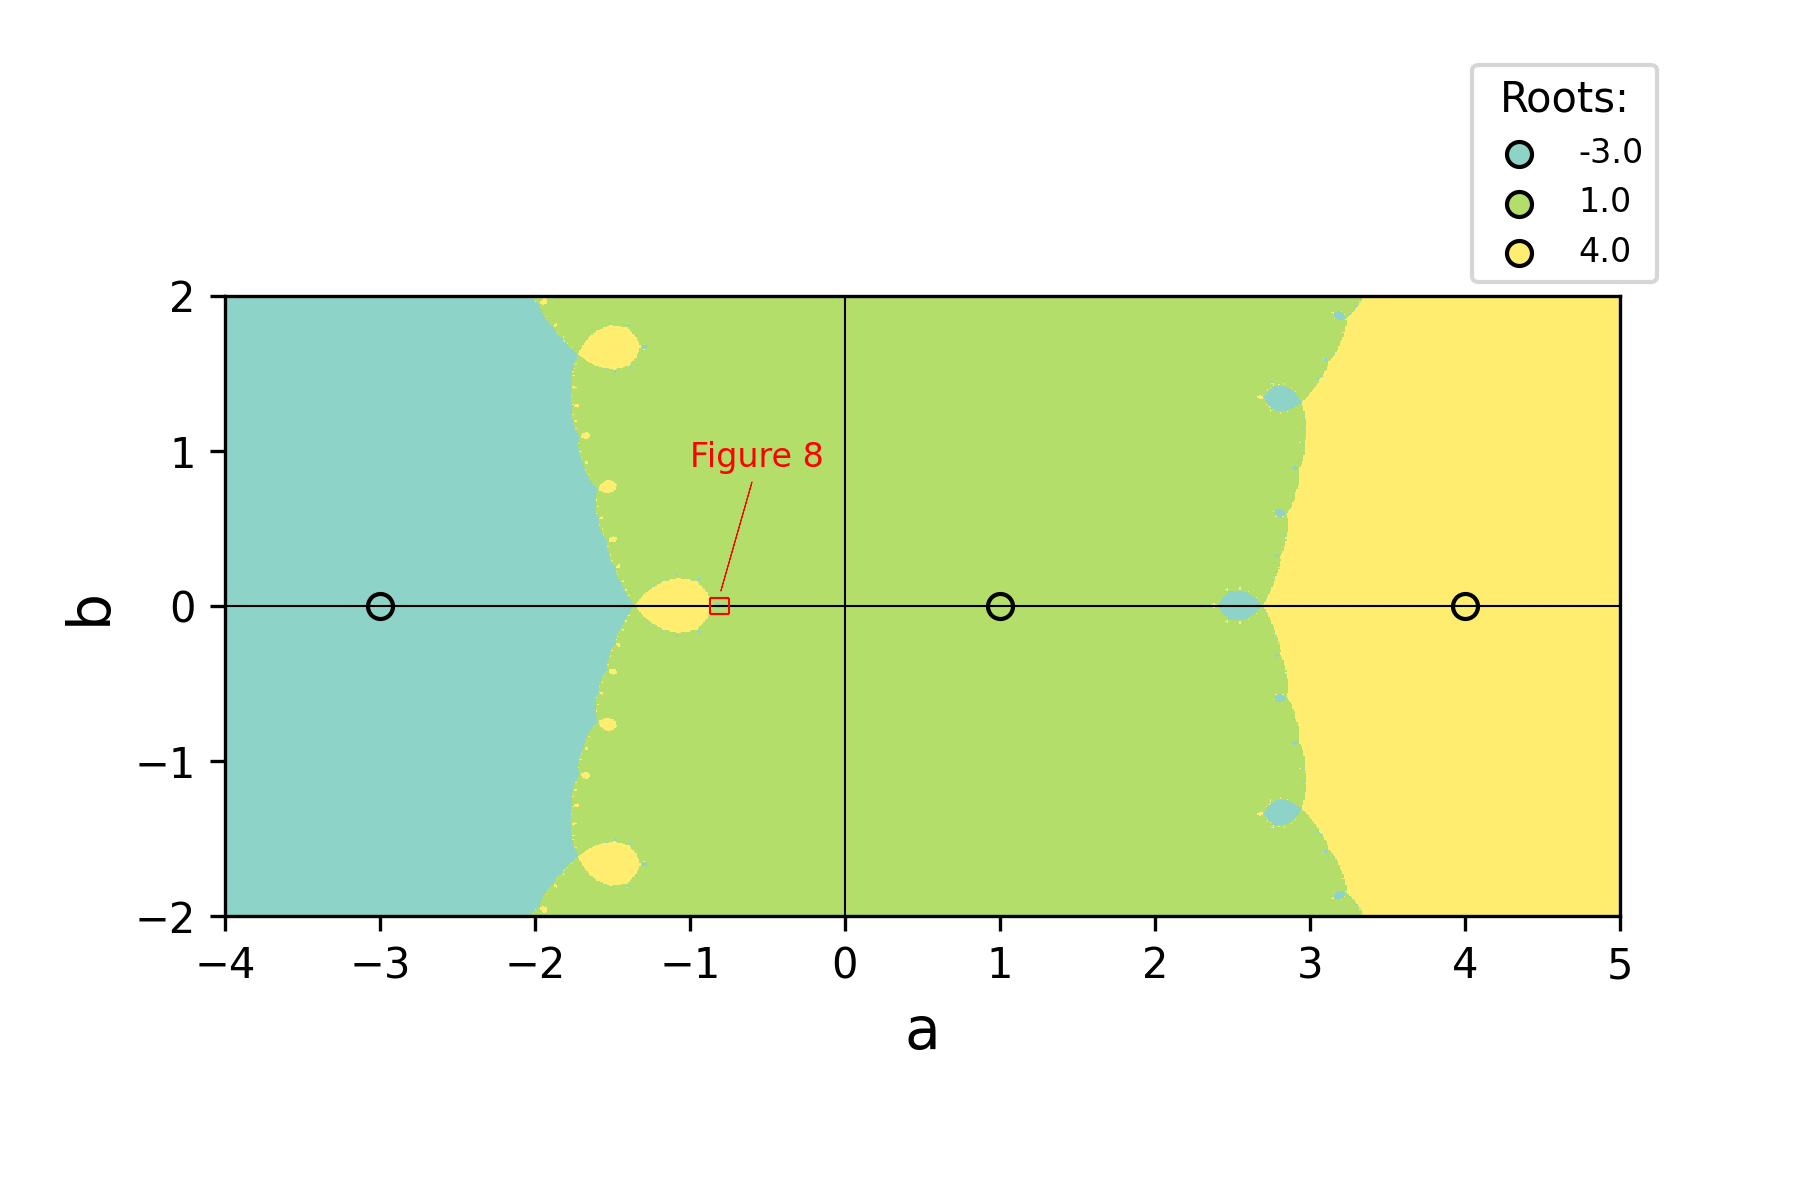
\includegraphics[scale=0.5]{figure7}
		\end{figure}
	
		\begin{figure}[H]
			\centering
			\caption{Zoom in on Figure 7 to show the fractal}
			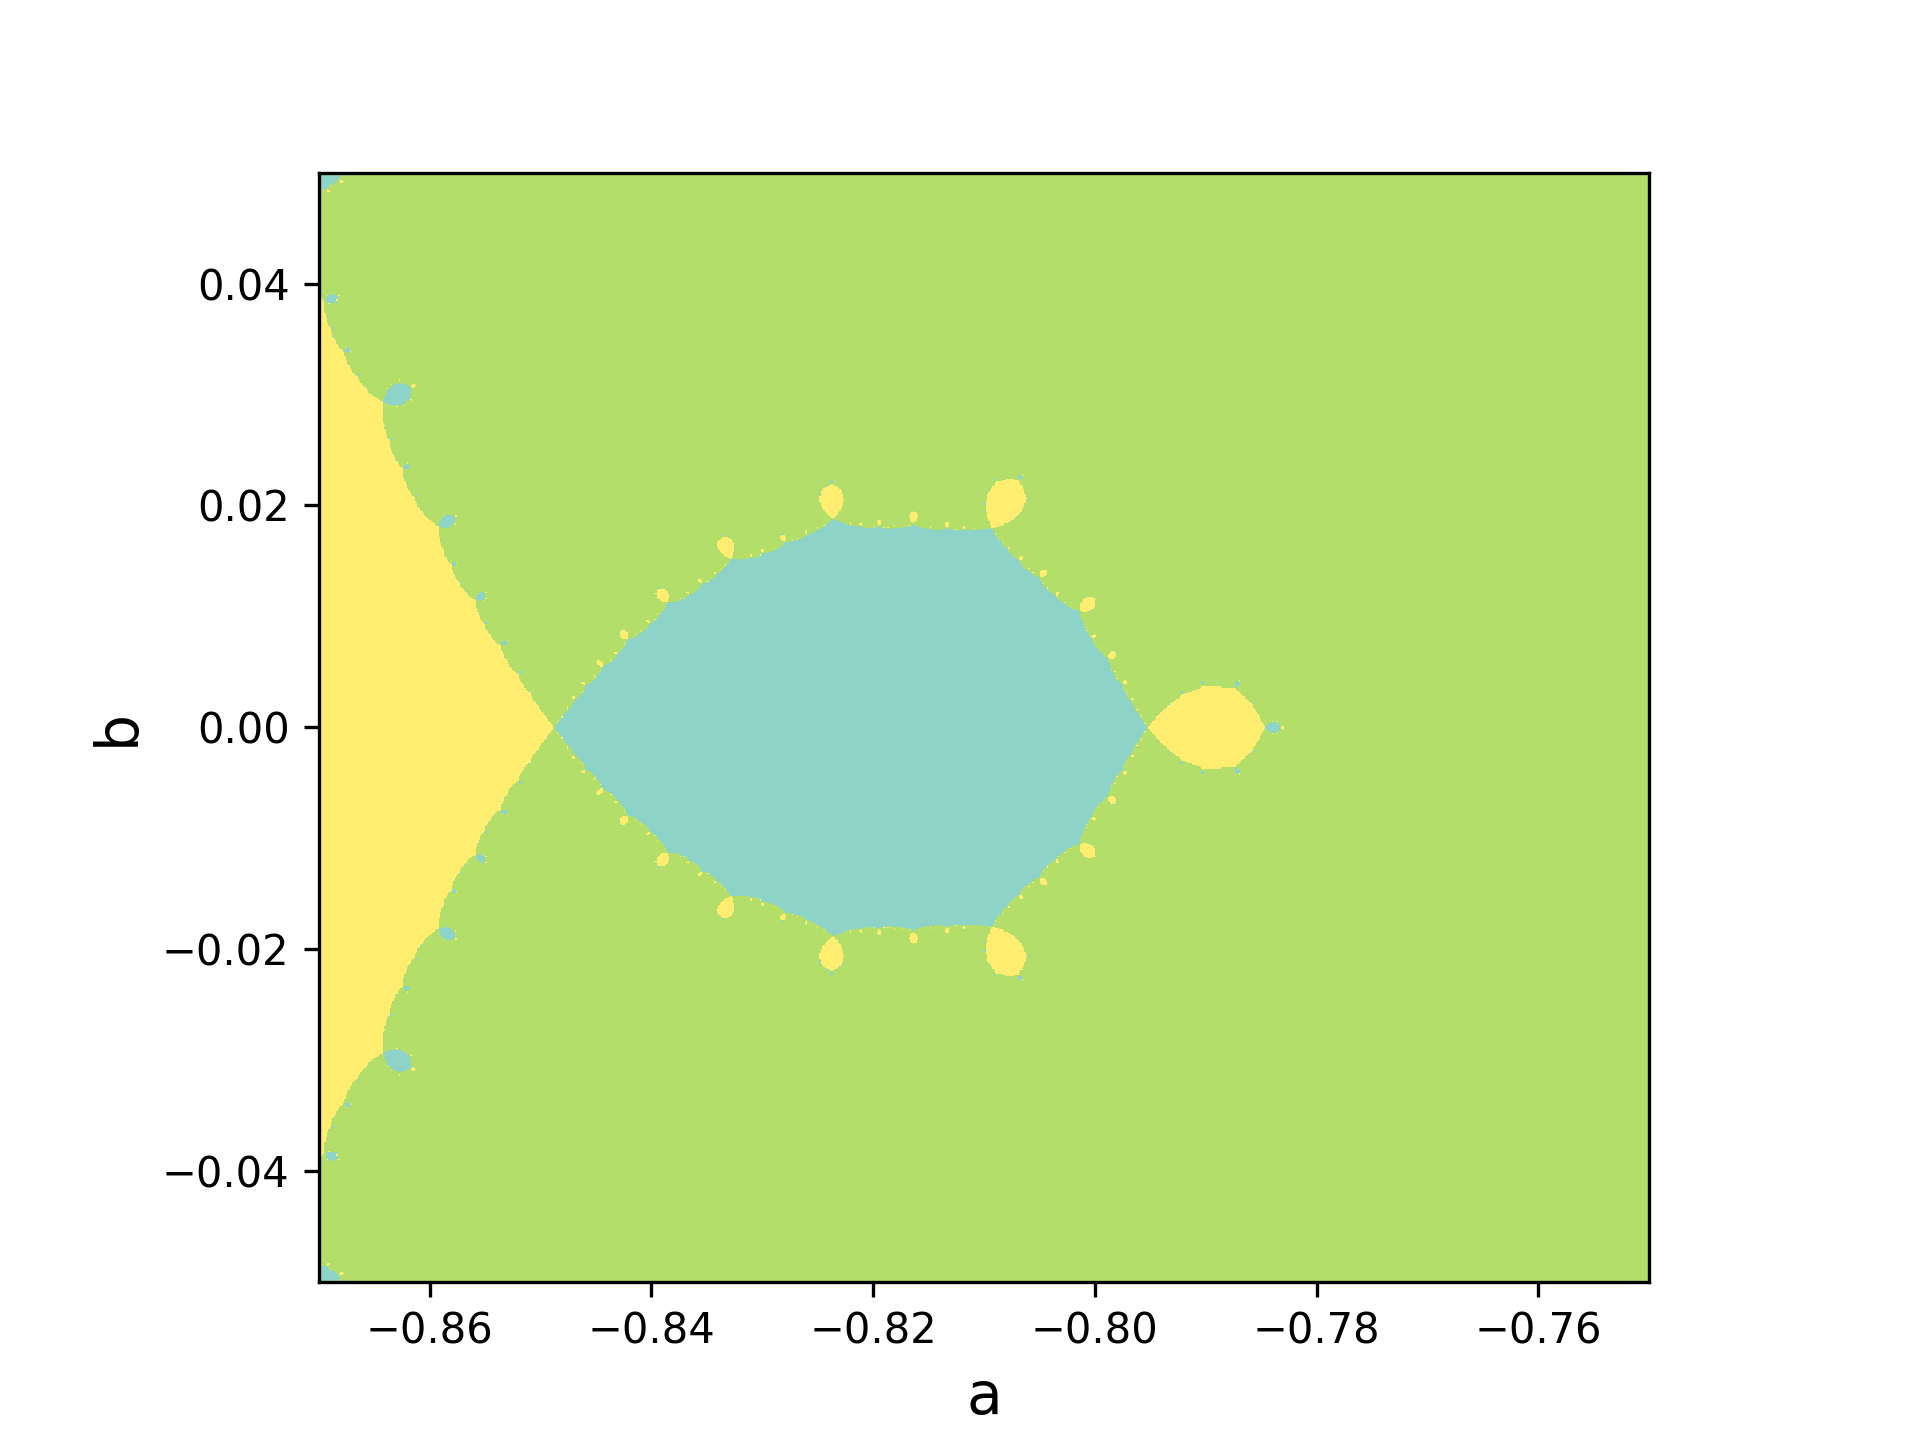
\includegraphics[scale=0.5]{figure8}
		\end{figure}
		
	\section{Discussion}
	In this project I examined the convergence of Newton's Method. First I looked at two functions for which Newton's Method does not converge. Then I visualized the basins of convergence for real- and complex-valued functions created by Newton's Method. For a function with at least three roots, the basins form fractals. I was somewhat surprised to find that the roots don't need to be complex, even three real roots will create fractal basins.
\end{document}